\documentclass[12pt, a4paper]{article}

\usepackage[czech]{babel}
\usepackage[IL2]{fontenc}
\usepackage[utf8]{inputenc}
\usepackage{lmodern}  % lepší kvalita PDF

\usepackage[a4paper,top=3cm,bottom=3cm,left=3cm,right=3cm,marginparwidth=1.75cm]{geometry}

\usepackage{graphicx}
\usepackage{titling}
\usepackage{enumitem}
\usepackage{caption}
\usepackage{float}
\usepackage{pdfpages}
\usepackage{verbatim}
\usepackage{amsmath}
\usepackage{multirow}

\usepackage{pkg-custom-commands}
\usepackage{pkg-url}

% údaje na titulní straně
\title{Cvičení 4}
\def \thesubtitle {KIV/VSS}
\author{Patrik Harag}
\def \theauthoremail {harag@students.zcu.cz}
\def \theauthorid {A18N0084P, nar. 10. května}

\begin{document}
	
	\begin{titlepage}
		\begin{figure}
			
\includegraphics[height=50mm]{img-fav-logo}
		\end{figure}
		
		\centering
		{\large \hspace{1mm} \par} % tady musí být nějaký text jinak nefunguje vertikální odsazení
		\vspace{15ex}
		
		{\huge\bfseries \thetitle \par}
		\vspace{2ex}
		{\scshape\Large \thesubtitle \par}
		\vspace{15ex}
		{\Large\itshape \theauthor \par}
		\vspace{2ex}
		{\texttt{\theauthoremail} \par}
		\vspace{1ex}
		{\texttt{\theauthorid} \par}
		
		\vfill
		
		{\today\par}
	\end{titlepage}
	
	\section*{Zadání}
	
	\paragraph{6.}
	Porovnejte rychlost operace toArray nad kolekcemi ArrayList a LinkedList s~dostatečným množstvím dat.
	
	\section*{Konfigurace prostředí}
	\paragraph{Hardware}
	\begin{itemize}
		\item Notebook Lenovo G510,
		\item Intel Core i3-4000M 2.40 GHz,
		\item 8 GB RAM,
		\item WD Green 3D NAND SSD 240GB 2.5".
	\end{itemize}
	
	\paragraph{Platforma}
	\begin{itemize}
		\item Windows 10 Pro, 64 bit (10.0.18362 Build 18362)
		\item JDK 1.8.0\_144
		\item Apache Maven 3.5.0
	\end{itemize}
	
	\section*{Způsob měření}
	Pro tvorbu benchmarku byl použit framework JMH.
	Konfigurace je kombinace velikosti kolekce (100 000, 1 000 000, 10 000 000) a typu kolekce (ArrayList, LinkedList, Vector).
	Kolekce se plní objekty typu Integer.
	Pro každou konfiguraci se provádí 5 warmup iterací a 10 měřených iterací. Iterace trvá 8 sekund. Celkem tedy benchmark trvá 18 minut.
	
	\section*{Výsledky}
	\begin{table}
		\scriptsize
		\caption{Průměrné doby vykonání metody toArray v milisekundách}
		\centering
		\label{tbl:results}
		\begin{tabular}{l|l|l|l|}
			\multirow{2}{*}{Kolekce} & \multicolumn{3}{c}{Velikost} \\
			& 100 000 & 1 000 000 & 10 000 000 \\
			\hline
			\hline
			java.util.ArrayList & 0.079 $\pm$ 0.001 & 1.039 $\pm$ 0.002 & 11.041 $\pm$ 1.005 \\
			java.util.LinkedList & 0.585 $\pm$ 0.004 & 11.675 $\pm$ 0.358 & 121.389 $\pm$ 0.098 \\
			java.util.Vector & 0.079 $\pm$ 0.001 & 1.042 $\pm$ 0.002 & 11.109 $\pm$ 1.105
		\end{tabular}
	\end{table}
	\begin{figure}
		\centering
		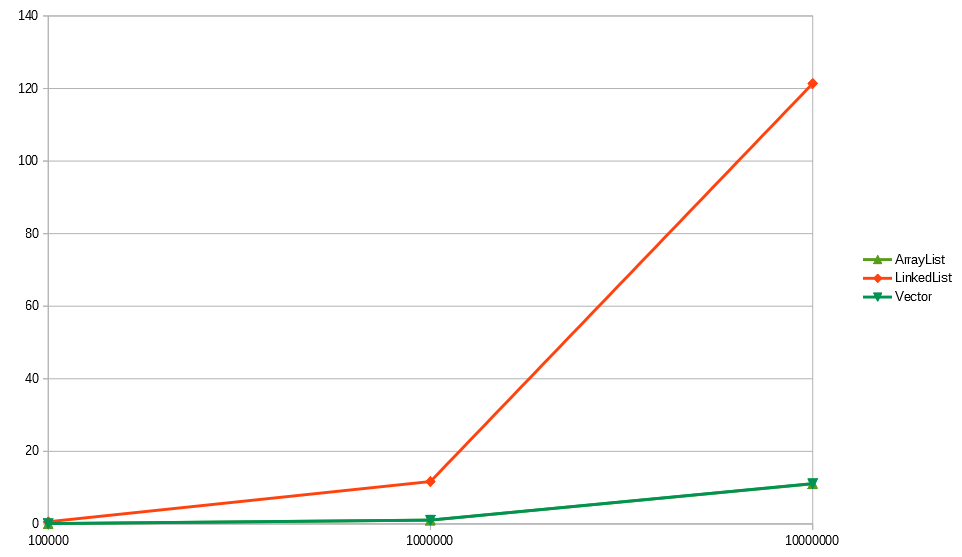
\includegraphics[width=1\linewidth]{chart}
		\caption{Průměrné doby vykonání metody toArray v milisekundách}
		\label{fig:chart}
	\end{figure}

	Výsledky měření jsou zobrazeny v Tabulce \ref{tbl:results}.
	Graf na Obrázku \ref{fig:chart} dále naměřené hodnoty vizualizuje.
	
	\section*{Závěr}
	Metoda toArray třídy java.util.ArrayList je rychlejší než metoda toArray třídy java.util.LinkedList, protože zkopírování bloku paměti je vždy rychlejší než iterace po prvcích a kopírování jedné hodnoty za druhou.
	Navíc byla změřena kolekce java.util.Vector, která dává, dle očekávání, podobné výsledky jako java.util.ArrayList. Téměř stejné jsou dokonce i odchylky.
	
	I přesto, že měření byla provedena pouze pro tři různé velikosti kolekce, lze výsledků v Tabulce \ref{tbl:results} pozorovat lineární závislost.
	Metoda toArray u kolekce s desetinásobným počtem prvků trvá vždy přibližně desetkrát tak dlouho.
	
\end{document}